\section{Results}\label{sec:results}

\begin{table}[h]
	\centering
	\begin{tabular}{|l|l|l|l|}
		\hline
		\textbf{Function Group} & \textbf{Dimension size}      & \textbf{Chi-squared}        & \textbf{P-value}                     \\ \hline
		\multicolumn{1}{|l|}{Unimodal} & \multicolumn{1}{|l|}{10} & \multicolumn{1}{l|}{24.955} & \multicolumn{1}{l|}{ 0.2992} \\ \hline
		\multicolumn{1}{|l|}{Multimodal} & \multicolumn{1}{|l|}{10} & \multicolumn{1}{l|}{66.904} & \multicolumn{1}{l|}{2.012e-06}  \\ \hline
		\hline
		\multicolumn{1}{|l|}{Unimodal} & \multicolumn{1}{|l|}{20} & \multicolumn{1}{l|}{20.24} & \multicolumn{1}{l|}{0.5681} \\ \hline
		\multicolumn{1}{|l|}{Multimodal} & \multicolumn{1}{|l|}{20} & \multicolumn{1}{l|}{57.525} & \multicolumn{1}{l|}{5.152e-05}  \\ \hline
		\hline	
		\multicolumn{1}{|l|}{Unimodal} & \multicolumn{1}{|l|}{40} & \multicolumn{1}{l|}{25.34} & \multicolumn{1}{l|}{0.2811} \\ \hline
		\multicolumn{1}{|l|}{Multimodal} & \multicolumn{1}{|l|}{40} & \multicolumn{1}{l|}{37.091} & \multicolumn{1}{l|}{0.02312}  \\ \hline
	\end{tabular}
	\caption{Friedman Test results for Uniform Crossover - ($\lambda, \lambda$) scheme.}
	\label{Friedman_test_uniform-a}	
\end{table}


\begin{table}[h]
	\centering
	\begin{tabular}{|l|l|l|l|}
		\hline
		\textbf{Function Group} & \textbf{Dimension size}      & \textbf{Chi-squared}        & \textbf{P-value}                     \\ \hline
		\multicolumn{1}{|l|}{Unimodal} & \multicolumn{1}{|l|}{10} & \multicolumn{1}{l|}{53.379} & \multicolumn{1}{l|}{0.0002011} \\ \hline
		\multicolumn{1}{|l|}{Multimodal} & \multicolumn{1}{|l|}{10} & \multicolumn{1}{l|}{81.653} & \multicolumn{1}{l|}{8.645e-09}  \\ \hline
		\hline
		\multicolumn{1}{|l|}{Unimodal} & \multicolumn{1}{|l|}{20} & \multicolumn{1}{l|}{113.02} & \multicolumn{1}{l|}{3.181e-14} \\ \hline
		\multicolumn{1}{|l|}{Multimodal} & \multicolumn{1}{|l|}{20} & \multicolumn{1}{l|}{88.885} & \multicolumn{1}{l|}{5.302e-10}  \\ \hline
		\hline
		\multicolumn{1}{|l|}{Unimodal} & \multicolumn{1}{|l|}{40} & \multicolumn{1}{l|}{163.13} & \multicolumn{1}{l|}{$>$ 2.2e-16} \\ \hline
		\multicolumn{1}{|l|}{Multimodal} & \multicolumn{1}{|l|}{40} & \multicolumn{1}{l|}{118.46} & \multicolumn{1}{l|}{3.316e-15}  \\ \hline
	\end{tabular}
	\caption{Friedman Test results for SBX Crossover - ($\lambda, \lambda$) scheme.}
	\label{Friedman_test_sbx-a}	
\end{table}

	

\begin{table}[h]
	\centering
	\begin{tabular}{|l|l|l|l|}
		\hline
		\textbf{Function Group} & \textbf{Dimension size}      & \textbf{Chi-squared}        & \textbf{P-value}                     \\ \hline
		\multicolumn{1}{|l|}{Unimodal} & \multicolumn{1}{|l|}{10} & \multicolumn{1}{l|}{54.011} & \multicolumn{1}{l|}{0.0001639} \\ \hline
		\multicolumn{1}{|l|}{Multimodal} & \multicolumn{1}{|l|}{10} & \multicolumn{1}{l|}{75.724} & \multicolumn{1}{l|}{8.073e-08}  \\ \hline
		\hline
		\multicolumn{1}{|l|}{Unimodal} & \multicolumn{1}{|l|}{20} & \multicolumn{1}{l|}{73.078} & \multicolumn{1}{l|}{2.15e-07} \\ \hline
		\multicolumn{1}{|l|}{Multimodal} & \multicolumn{1}{|l|}{20} & \multicolumn{1}{l|}{95.524} & \multicolumn{1}{l|}{3.867e-11}  \\ \hline
		\hline
		\multicolumn{1}{|l|}{Unimodal} & \multicolumn{1}{|l|}{40} & \multicolumn{1}{l|}{115.38} & \multicolumn{1}{l|}{1.198e-14} \\ \hline
		\multicolumn{1}{|l|}{Multimodal} & \multicolumn{1}{|l|}{40} & \multicolumn{1}{l|}{87.318} & \multicolumn{1}{l|}{9.762e-10}  \\ \hline
	\end{tabular}
	\caption{Friedman Test results for SBX Crossover - ($\lambda + \lambda$) scheme.}
	\label{Friedman_test_sbx-b}	
\end{table}



\begin{figure*}[!t]
%	\Large{Average performance on different tournament size - Gallagher's Gaussian 21-hi Peaks Function}
	\begin{subfigure}[b]{0.33\textwidth}
		\centering
		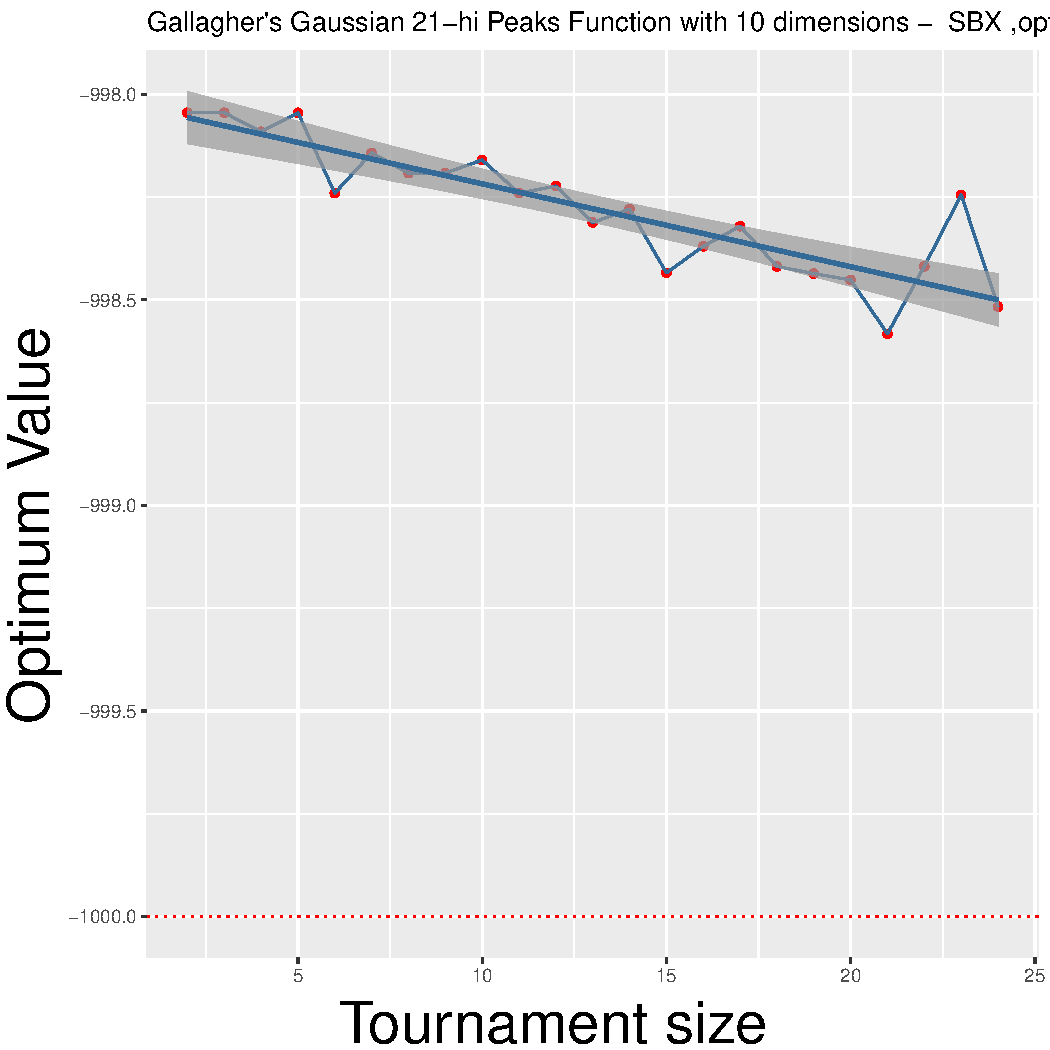
\includegraphics[width=\textwidth]{img/SBX-10D/multimodal_sbx_22_dim_10.pdf}
		\caption{Gallagher's Gaussian 21-hi Peaks Function - 10 dimensions.}
	\end{subfigure}
	\begin{subfigure}[b]{0.33\textwidth}
		\centering
		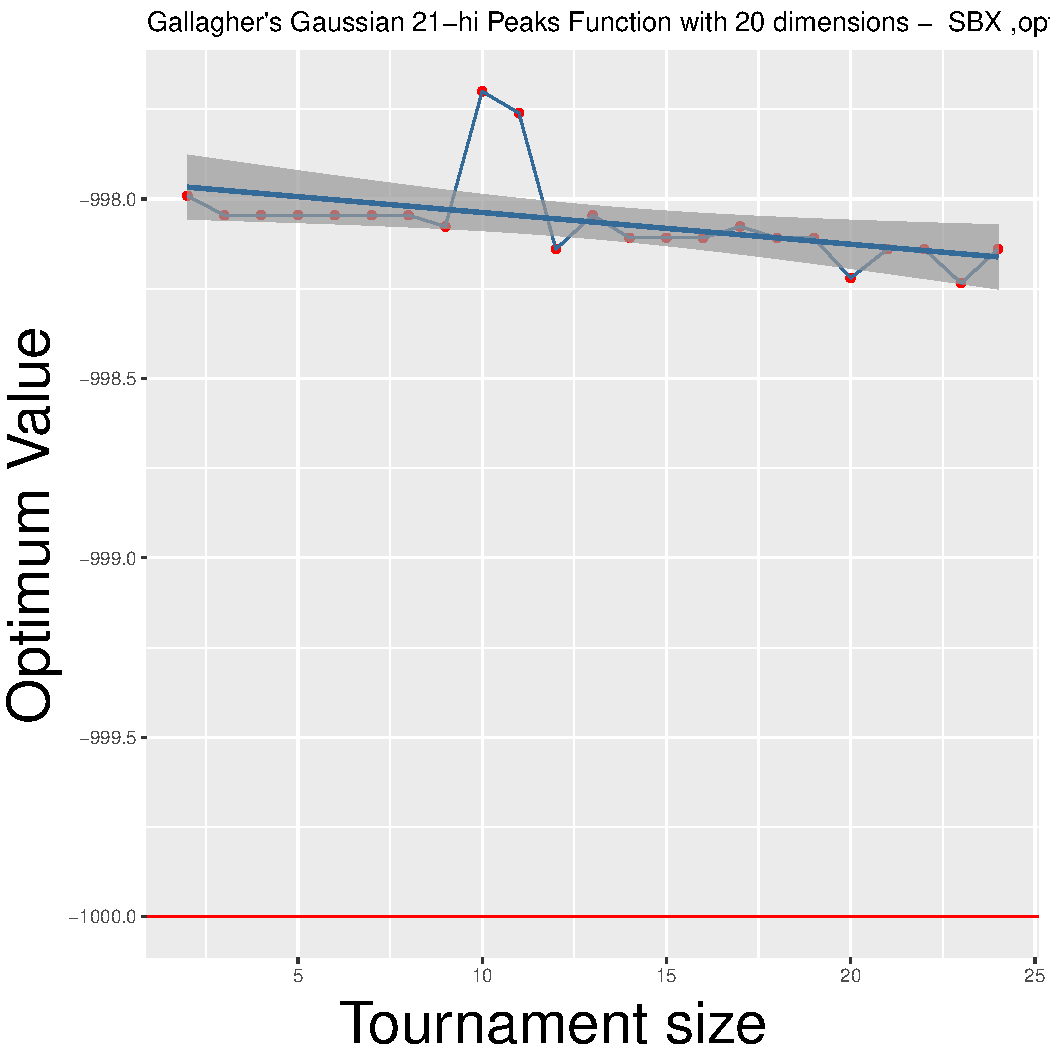
\includegraphics[width=\textwidth]{img/SBX-20D/multimodal_sbx_22_dim_20.pdf}
		\caption{Gallagher's Gaussian 21-hi Peaks Function - 20 dimensions.}
	\end{subfigure}
	\begin{subfigure}[b]{0.33\textwidth}
		\centering
		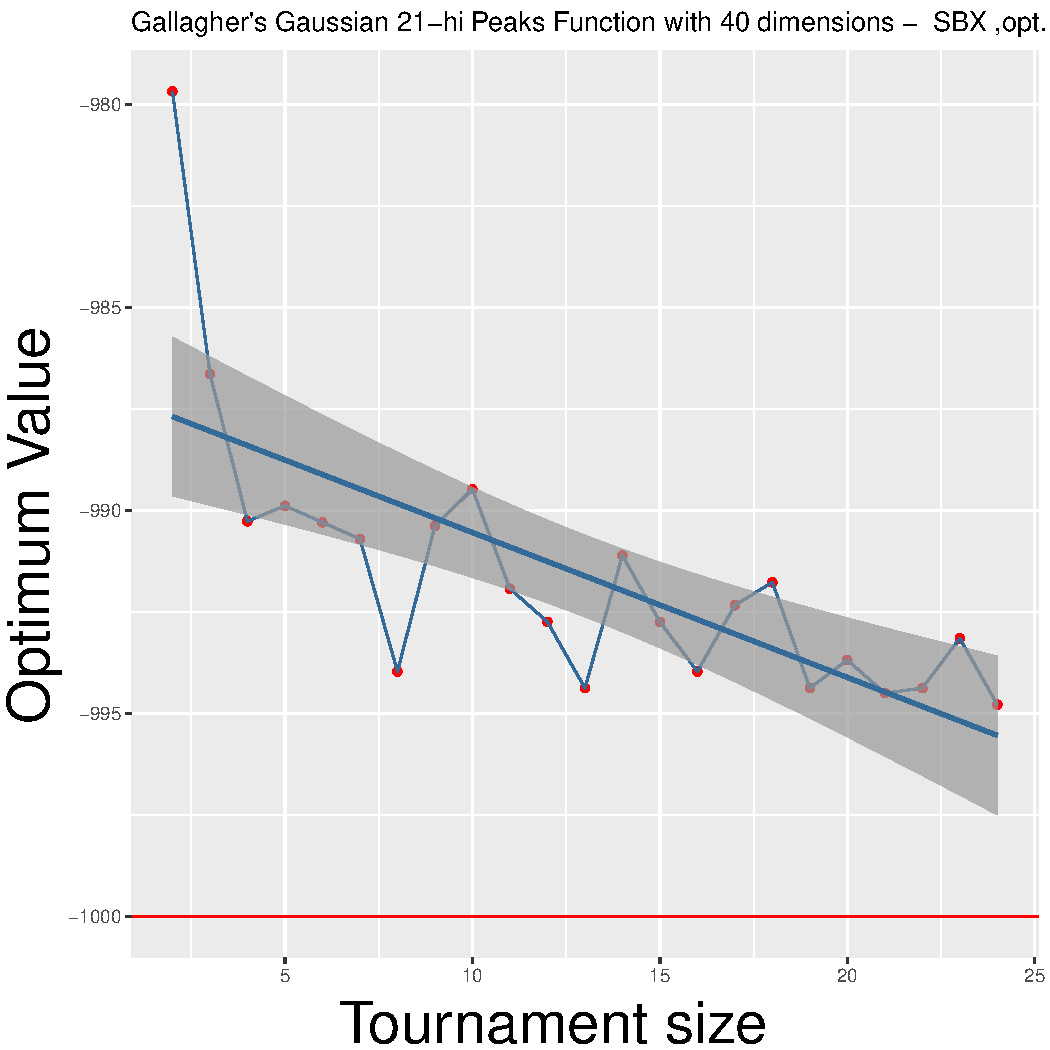
\includegraphics[width=\textwidth]{img/SBX-40D/multimodal_sbx_22_dim_40.pdf}
		\caption{Gallagher's Gaussian 21-hi Peaks Function - 40 dimensions.}
	\end{subfigure}
	\caption{SBX crossover - ($\lambda, \lambda$) scheme.}
	\label{sbx-22-a}
	\begin{subfigure}[b]{0.33\textwidth}
		\centering
		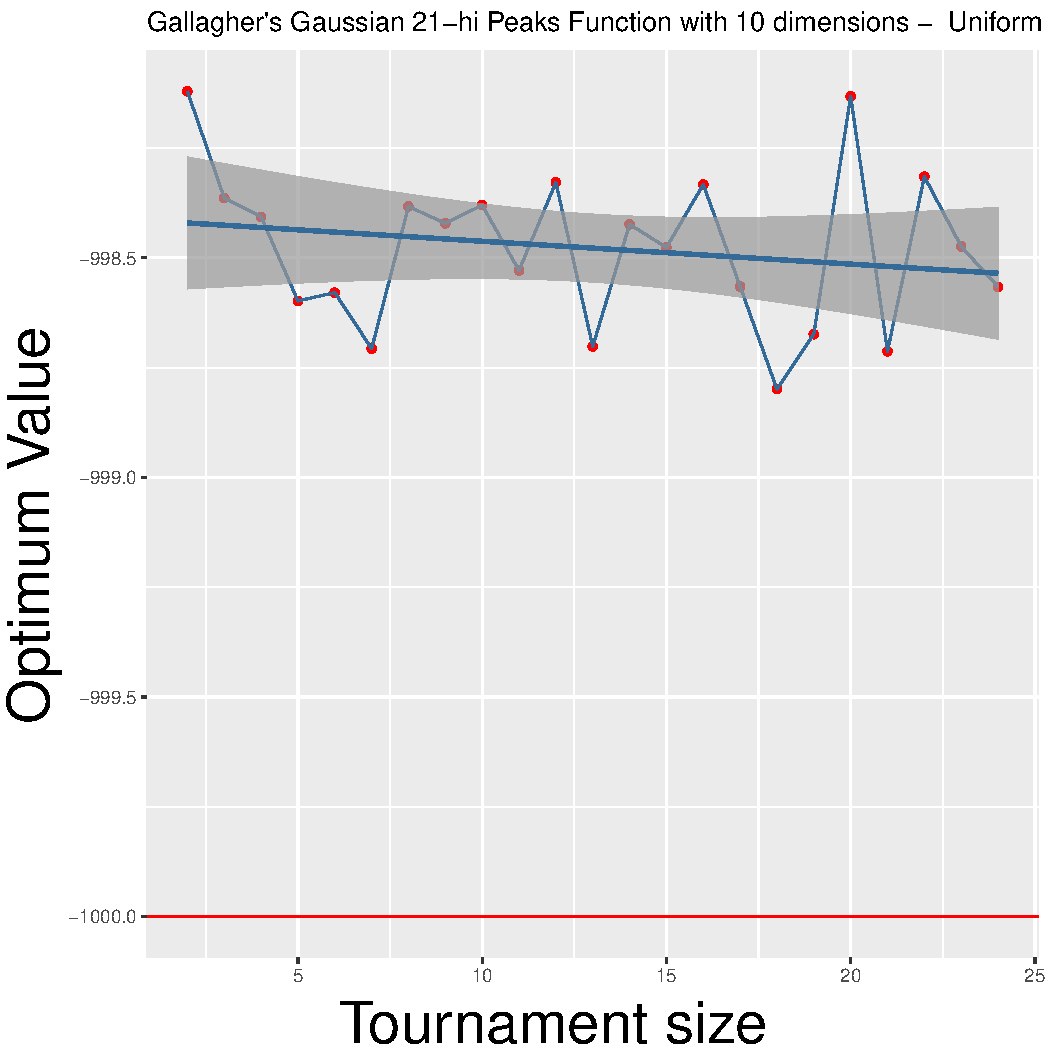
\includegraphics[width=\textwidth]{img/uniform-10D/multimodal_uniform_22_dim_10.pdf}
		\caption{Gallagher's Gaussian 21-hi Peaks Function - 10 dimensions.}
	\end{subfigure}
	\begin{subfigure}[b]{0.33\textwidth}
		\centering
		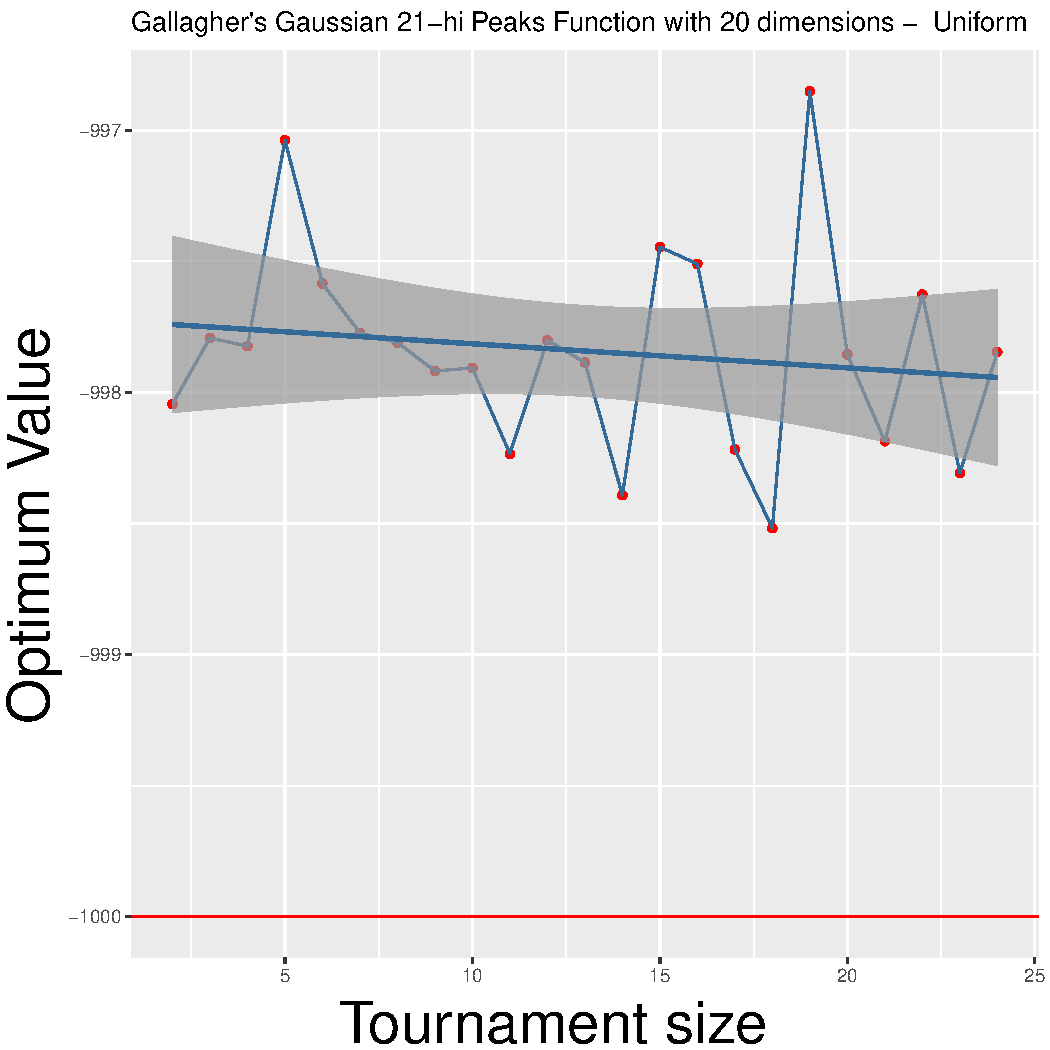
\includegraphics[width=\textwidth]{img/uniform-20D/multimodal_uniform_22_dim_20.pdf}
		\caption{Gallagher's Gaussian 21-hi Peaks Function - 20 dimensions.}
	\end{subfigure}
	\begin{subfigure}[b]{0.33\textwidth}
		\centering
		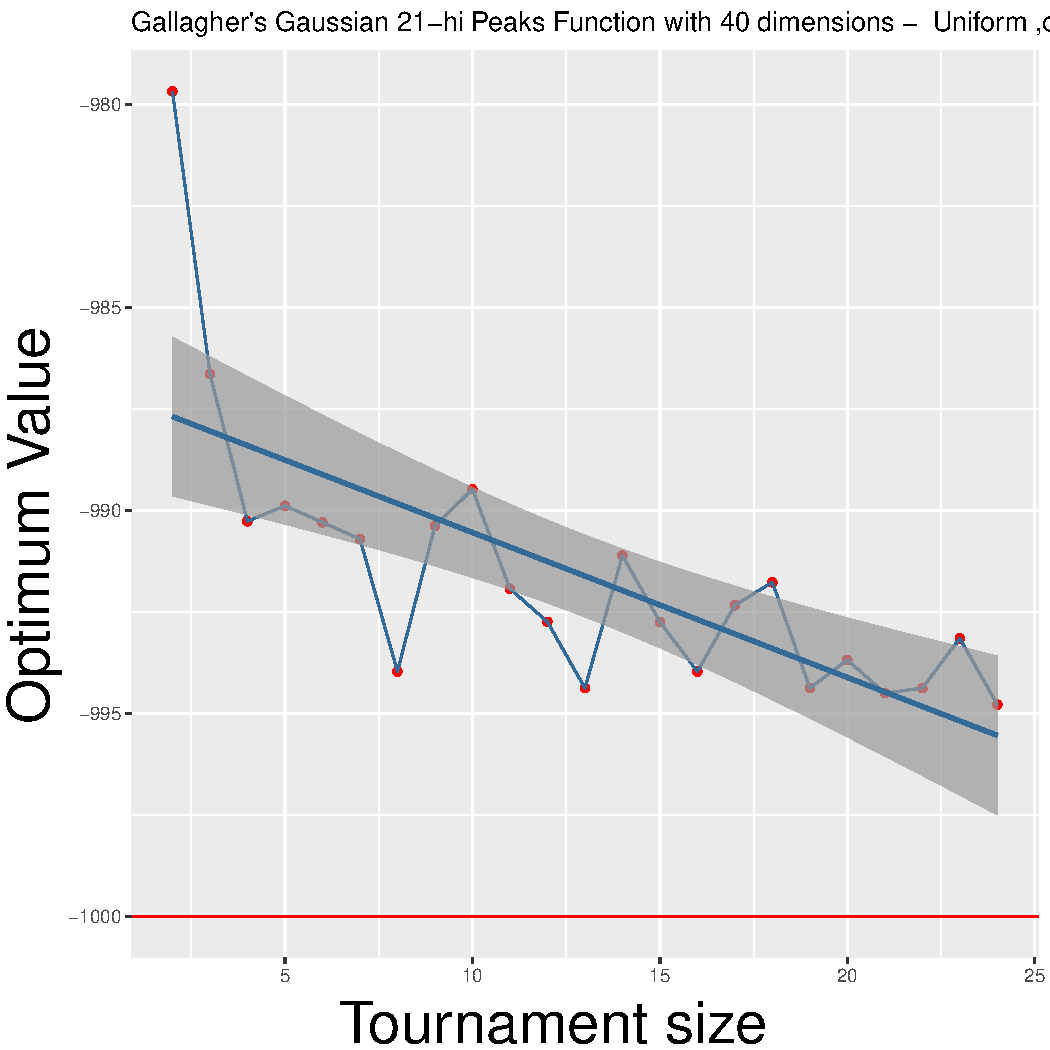
\includegraphics[width=\textwidth]{img/uniform-40D/multimodal_uniform_22_dim_40.pdf}
		\caption{Gallagher's Gaussian 21-hi Peaks Function - 40 dimensions.}
	\end{subfigure}
	\caption{Uniform crossover - ($\lambda, \lambda$) scheme.}
	\label{uniform-22-a}
	\begin{subfigure}[b]{0.33\textwidth}
		\centering
		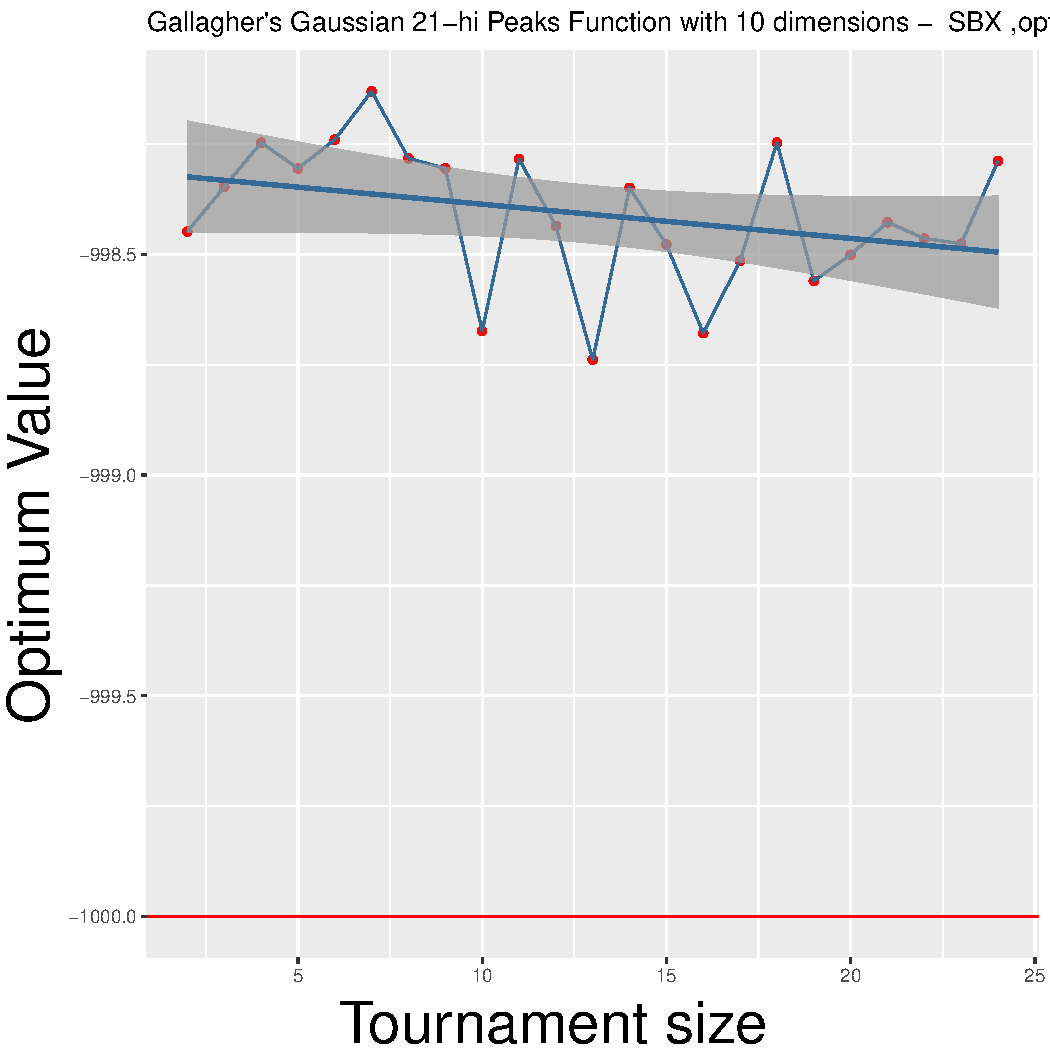
\includegraphics[width=\textwidth]{img/2n2n-10D/multimodal_2n2n_22_dim_10.pdf}
		\caption{Gallagher's Gaussian 21-hi Peaks Function - 10 dimensions.}
	\end{subfigure}
	\begin{subfigure}[b]{0.33\textwidth}
		\centering
		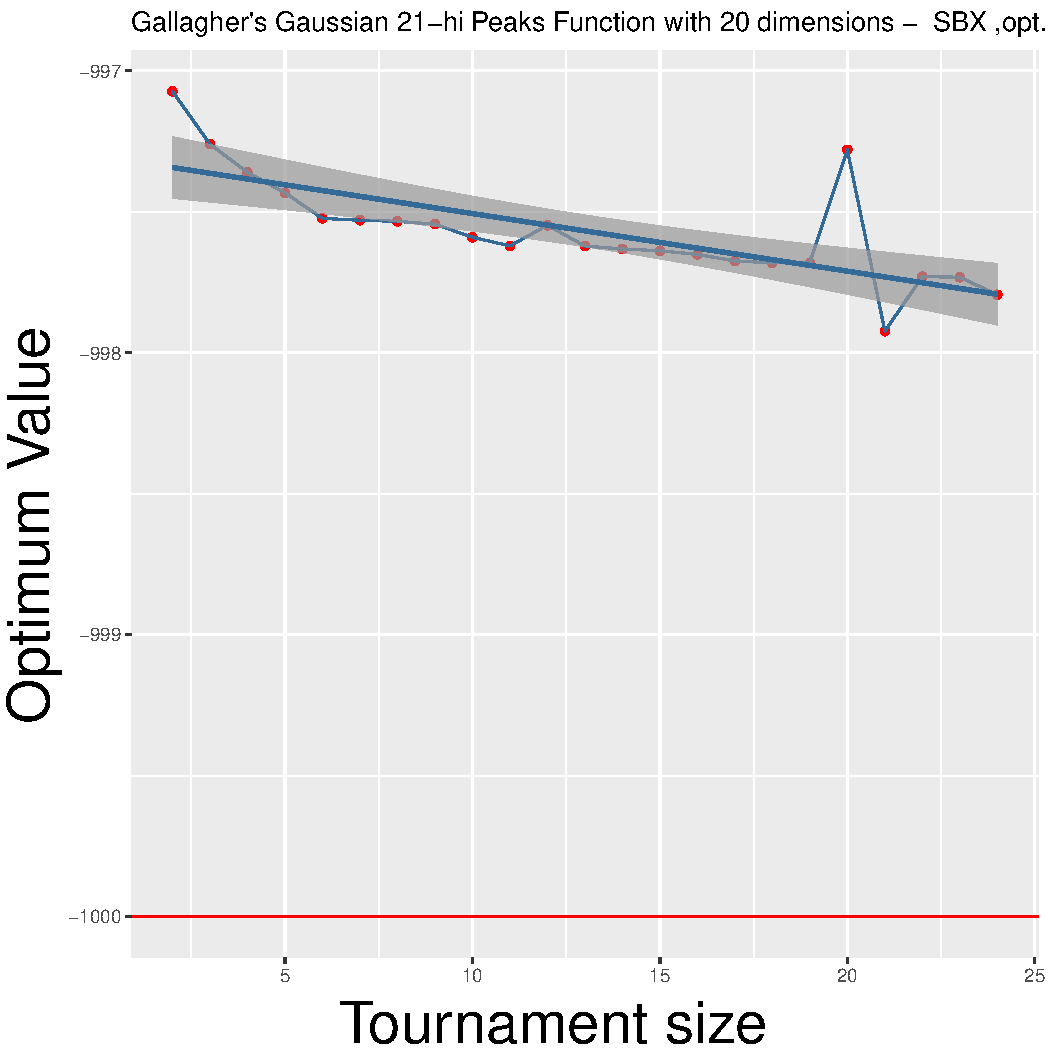
\includegraphics[width=\textwidth]{img/2n2n-20D/multimodal_2n2n_22_dim_20.pdf}
		\caption{Gallagher's Gaussian 21-hi Peaks Function - 20 dimensions.}
	\end{subfigure}
	\begin{subfigure}[b]{0.33\textwidth}
		\centering
		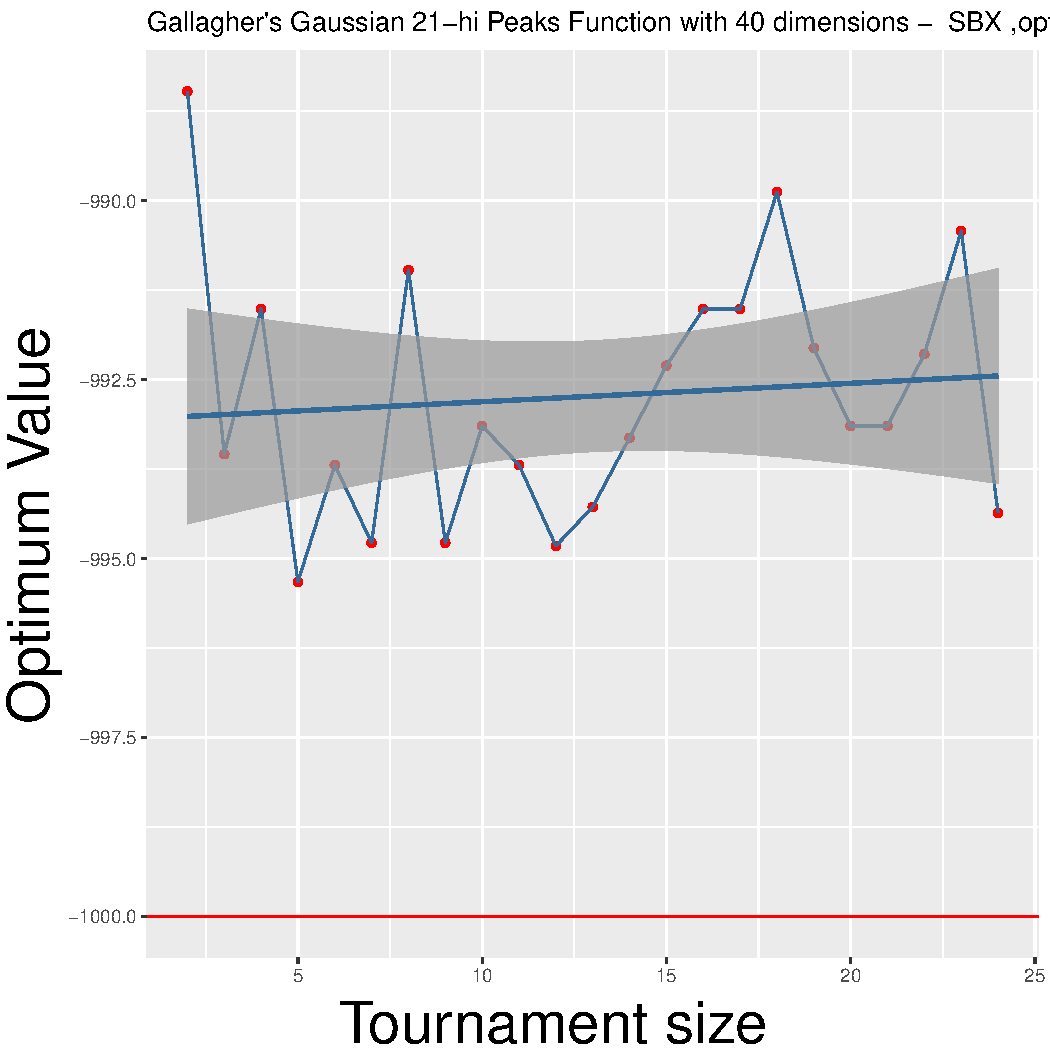
\includegraphics[width=\textwidth]{img/2n2n-40D/multimodal_2n2n_22_dim_40.pdf}
		\caption{Gallagher's Gaussian 21-hi Peaks Function - 40 dimensions.}
	\end{subfigure}
	\caption{SBX crossover - ($\lambda + \lambda$) scheme.}
	\label{sbx-22-B}
\end{figure*}


\begin{figure*}[!t]
	\begin{subfigure}[b]{0.33\textwidth}
		\centering
		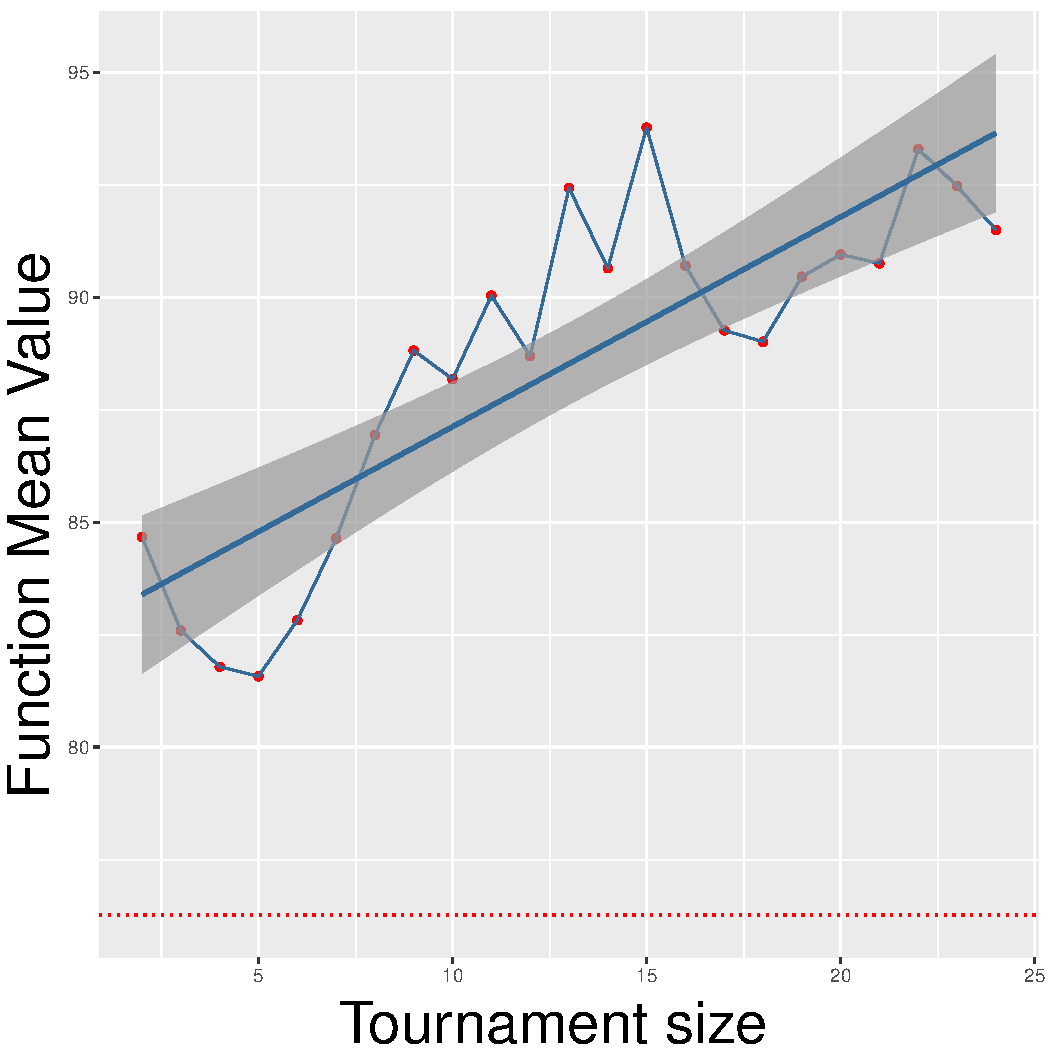
\includegraphics[width=\textwidth]{img/SBX-10D/unimodal_sbx_11_dim_10.pdf}
		\caption{Discus Function - 10 dimensions.}
	\end{subfigure}
	\begin{subfigure}[b]{0.33\textwidth}
		\centering
		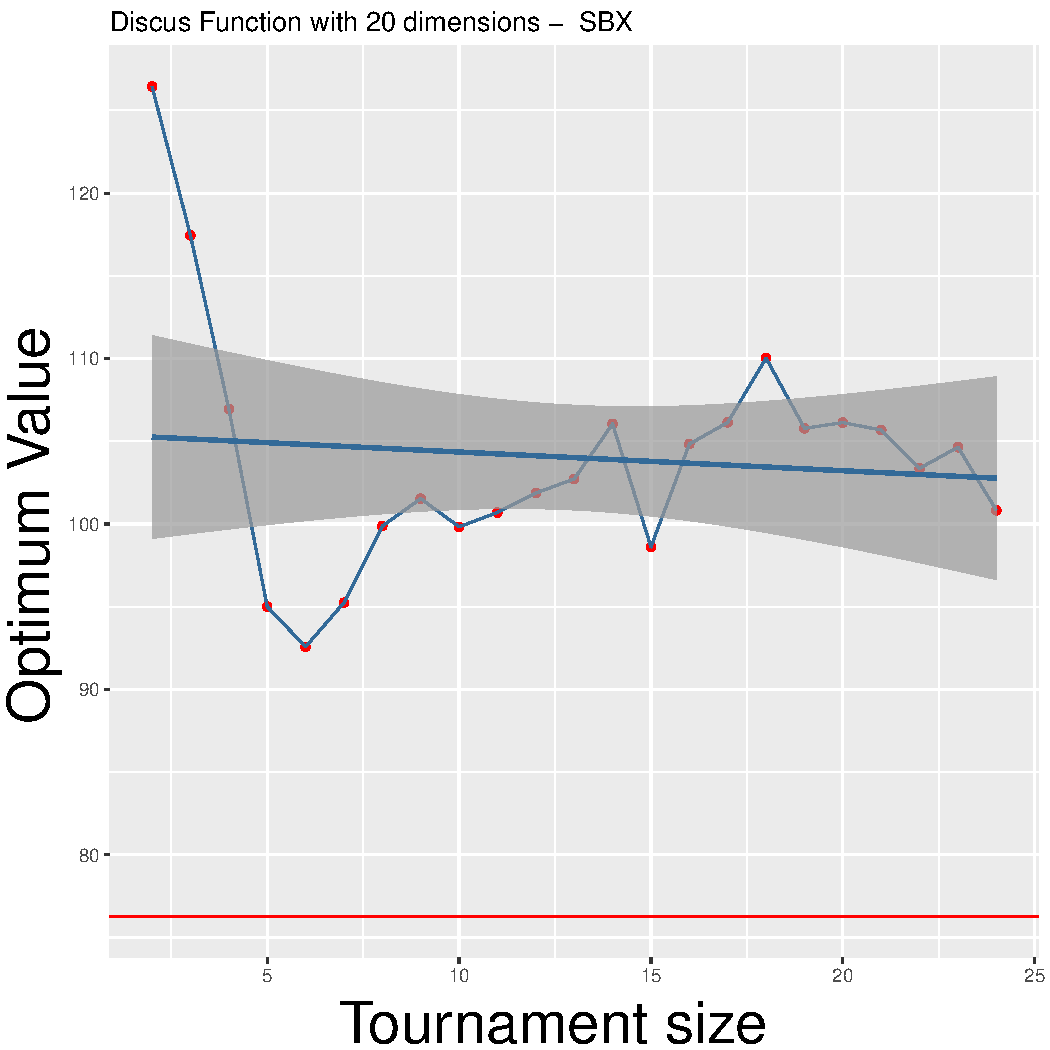
\includegraphics[width=\textwidth]{img/SBX-20D/unimodal_sbx_11_dim_20.pdf}
		\caption{Discus Function - 20 dimensions.}
	\end{subfigure}
	\begin{subfigure}[b]{0.33\textwidth}
		\centering
		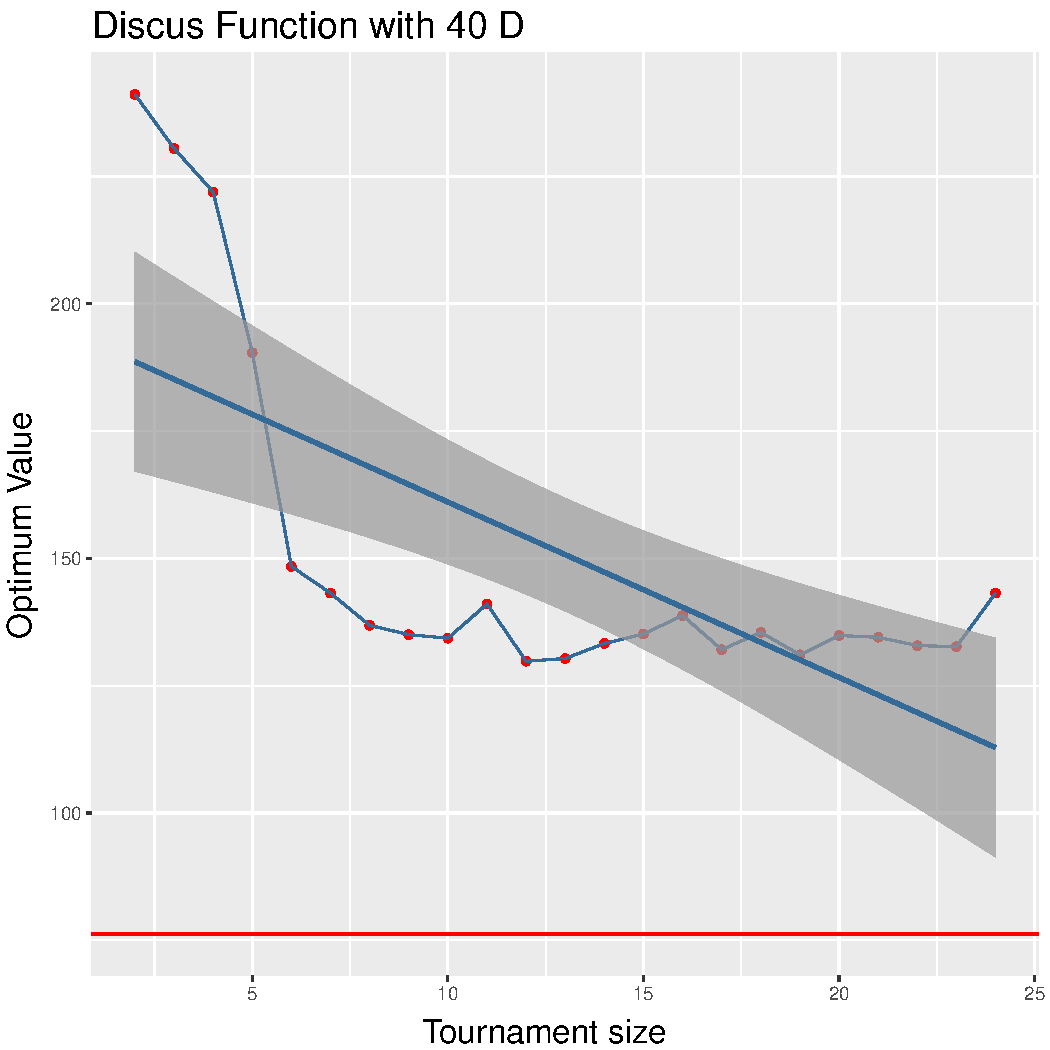
\includegraphics[width=\textwidth]{img/SBX-40D/unimodal_sbx_11_dim_40.pdf}
		\caption{Discus Function - 40 dimensions.}
	\end{subfigure}
	\caption{SBX crossover - ($\lambda, \lambda$) scheme.}
	\label{sbx-11-a}
	\begin{subfigure}[b]{0.33\textwidth}
		\centering
		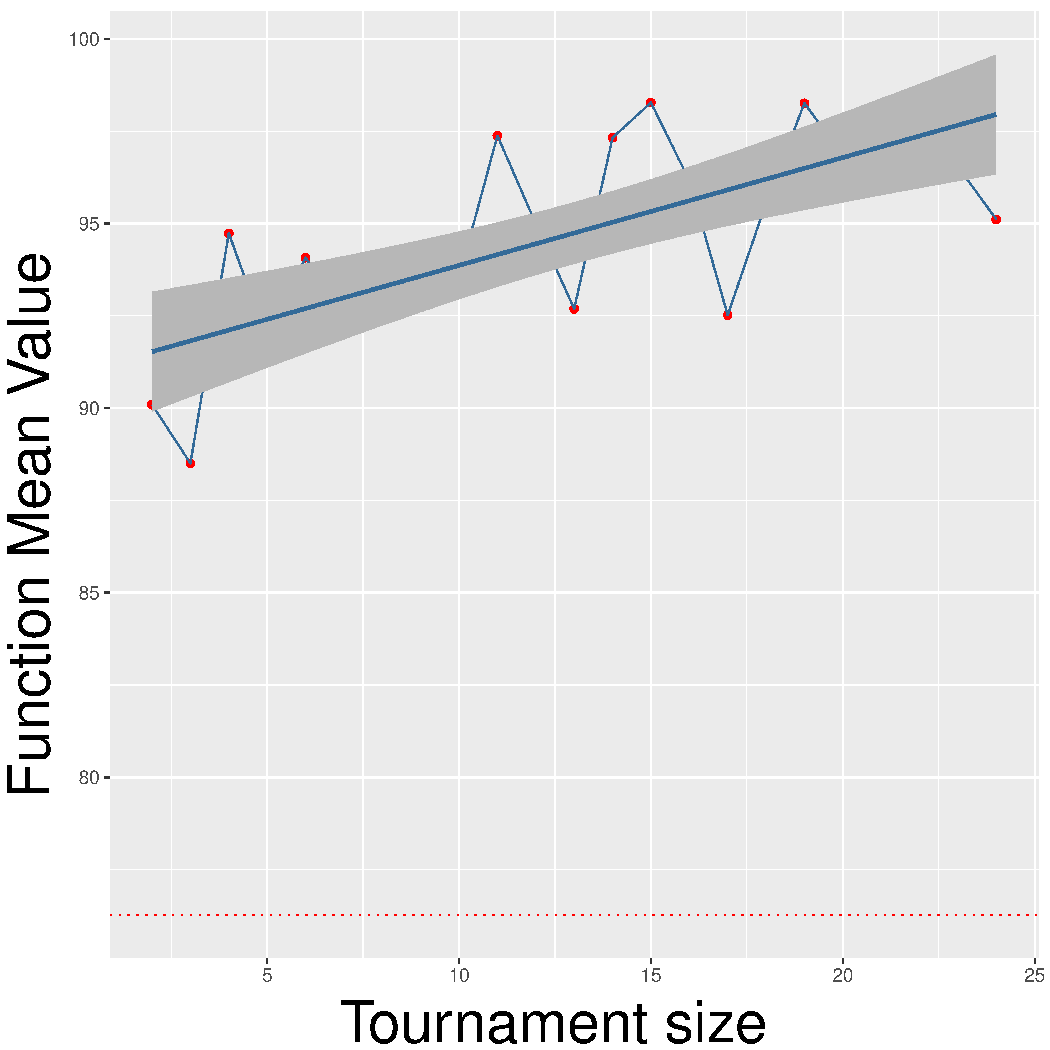
\includegraphics[width=\textwidth]{img/uniform-10D/unimodal_uniform_11_dim_10.pdf}
		\caption{Discus Function - 10 dimensions.}
	\end{subfigure}
	\begin{subfigure}[b]{0.33\textwidth}
		\centering
		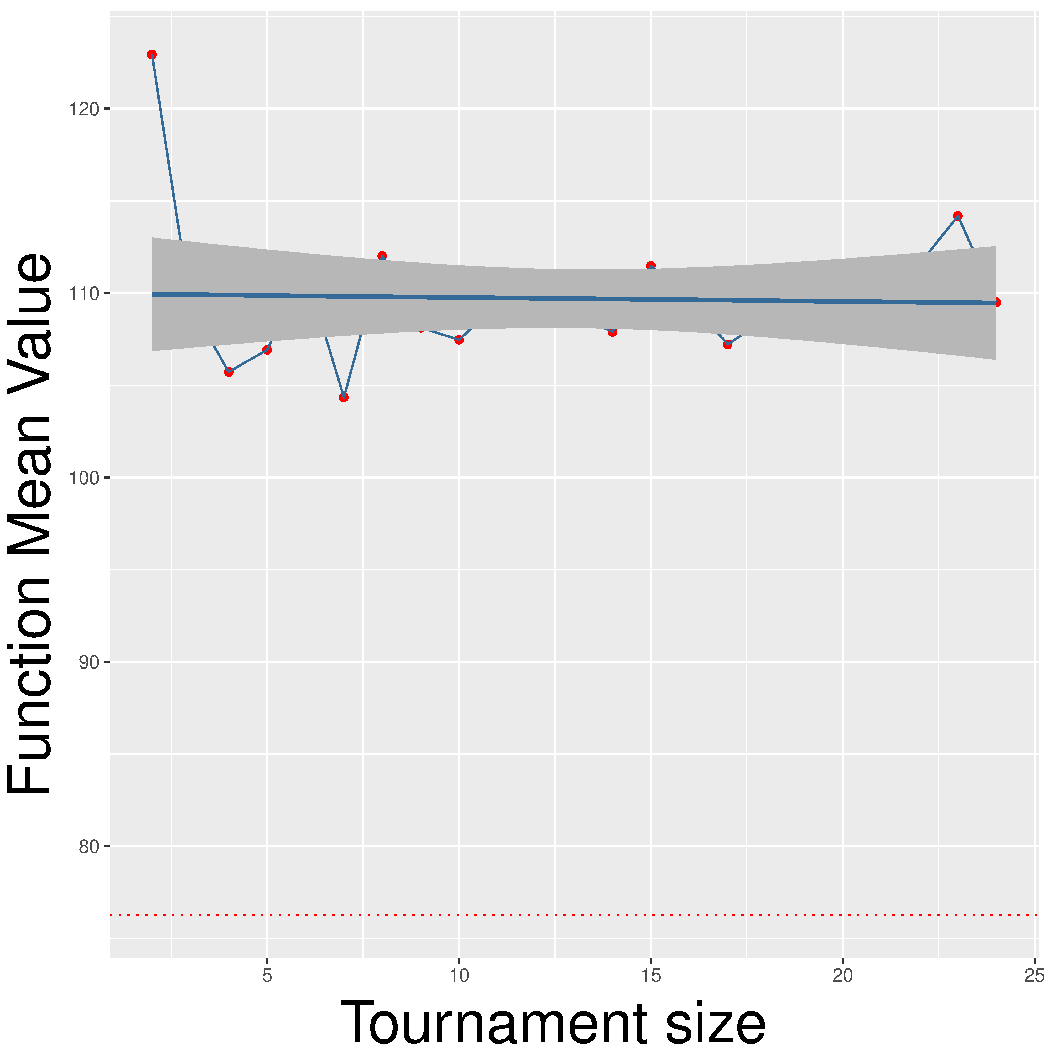
\includegraphics[width=\textwidth]{img/uniform-20D/unimodal_uniform_11_dim_20.pdf}
		\caption{Discus Function - 20 dimensions.}
	\end{subfigure}
	\begin{subfigure}[b]{0.33\textwidth}
		\centering
		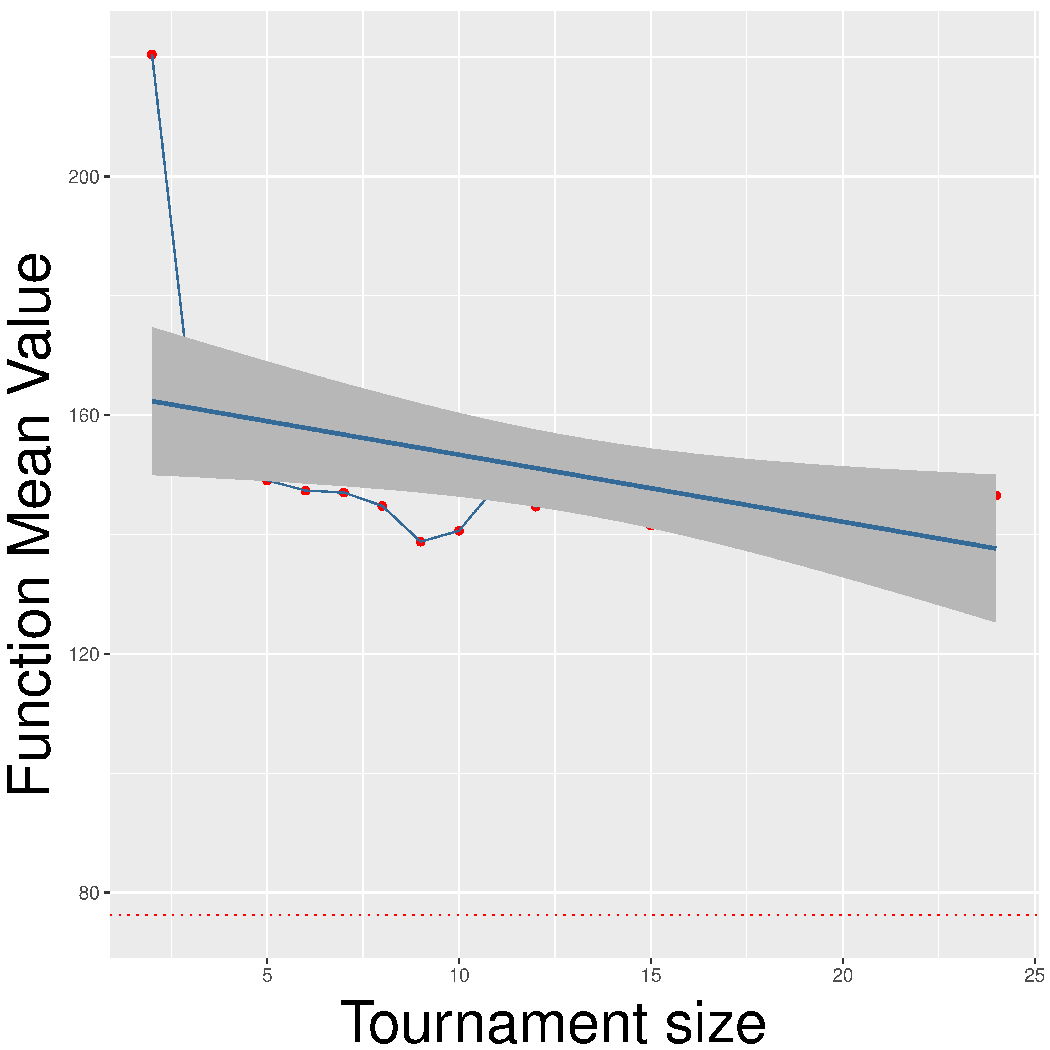
\includegraphics[width=\textwidth]{img/uniform-40D/unimodal_uniform_11_dim_40.pdf}
		\caption{Discus Function - 40 dimensions.}
	\end{subfigure}
	\caption{Uniform crossover - ($\lambda, \lambda$) scheme.}
	\label{uniform-11-a}
	\begin{subfigure}[b]{0.33\textwidth}
		\centering
		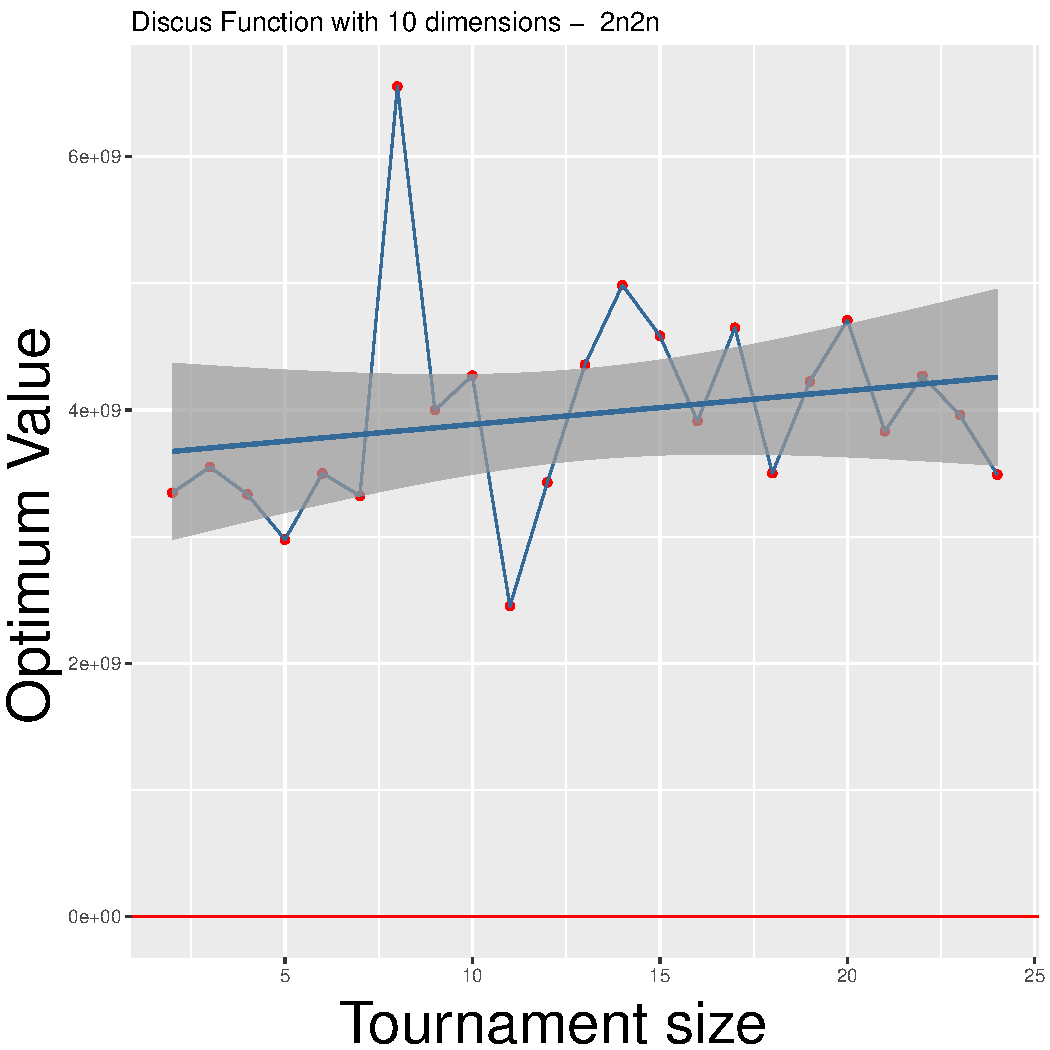
\includegraphics[width=\textwidth]{img/2n2n-10D/unimodal_2n2n_11_dim_10.pdf}
		\caption{Discus Function - 10 dimensions.}
	\end{subfigure}
	\begin{subfigure}[b]{0.33\textwidth}
		\centering
		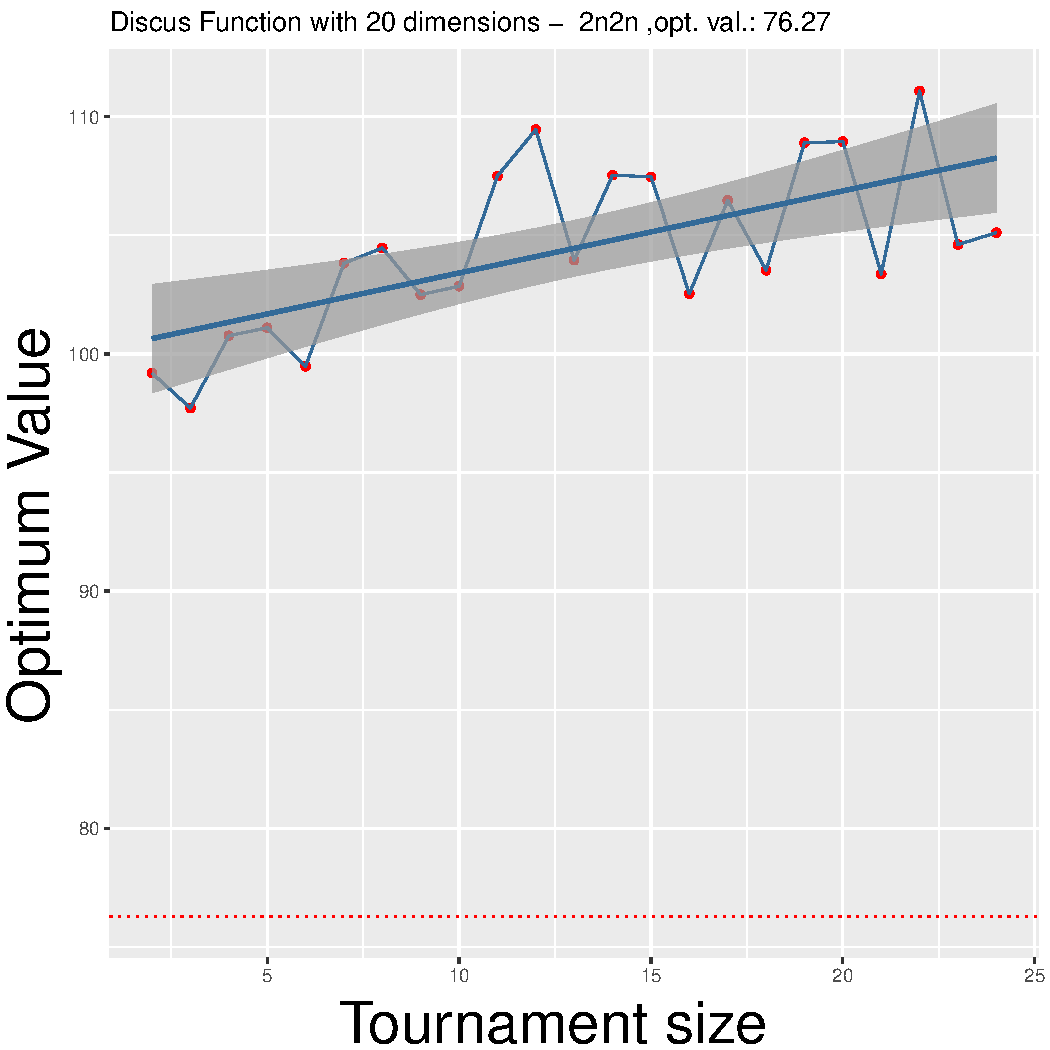
\includegraphics[width=\textwidth]{img/2n2n-20D/unimodal_2n2n_11_dim_20.pdf}
		\caption{Discus Function - 20 dimensions.}
	\end{subfigure}
	\begin{subfigure}[b]{0.33\textwidth}
		\centering
		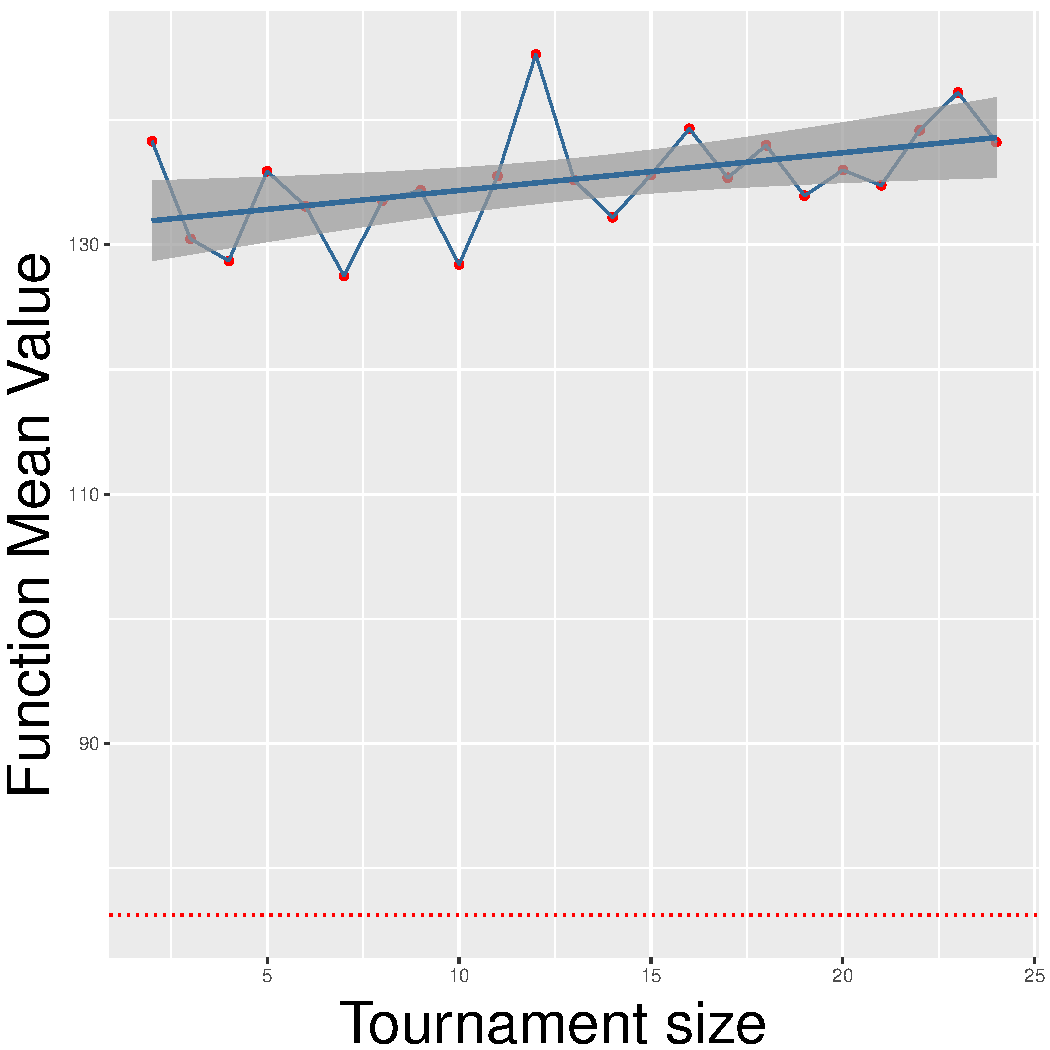
\includegraphics[width=\textwidth]{img/2n2n-40D/unimodal_2n2n_11_dim_40.pdf}
		\caption{Discus Function - 40 dimensions.}
	\end{subfigure}
	\caption{SBX crossover - ($\lambda + \lambda$) scheme.}
	\label{sbx-11-B}
\end{figure*}


\begin{figure*}[!t]
%	\captionsetup{format = hang, justification = raggedright}
	\begin{subfigure}[b]{0.24\textwidth}
		\centering
		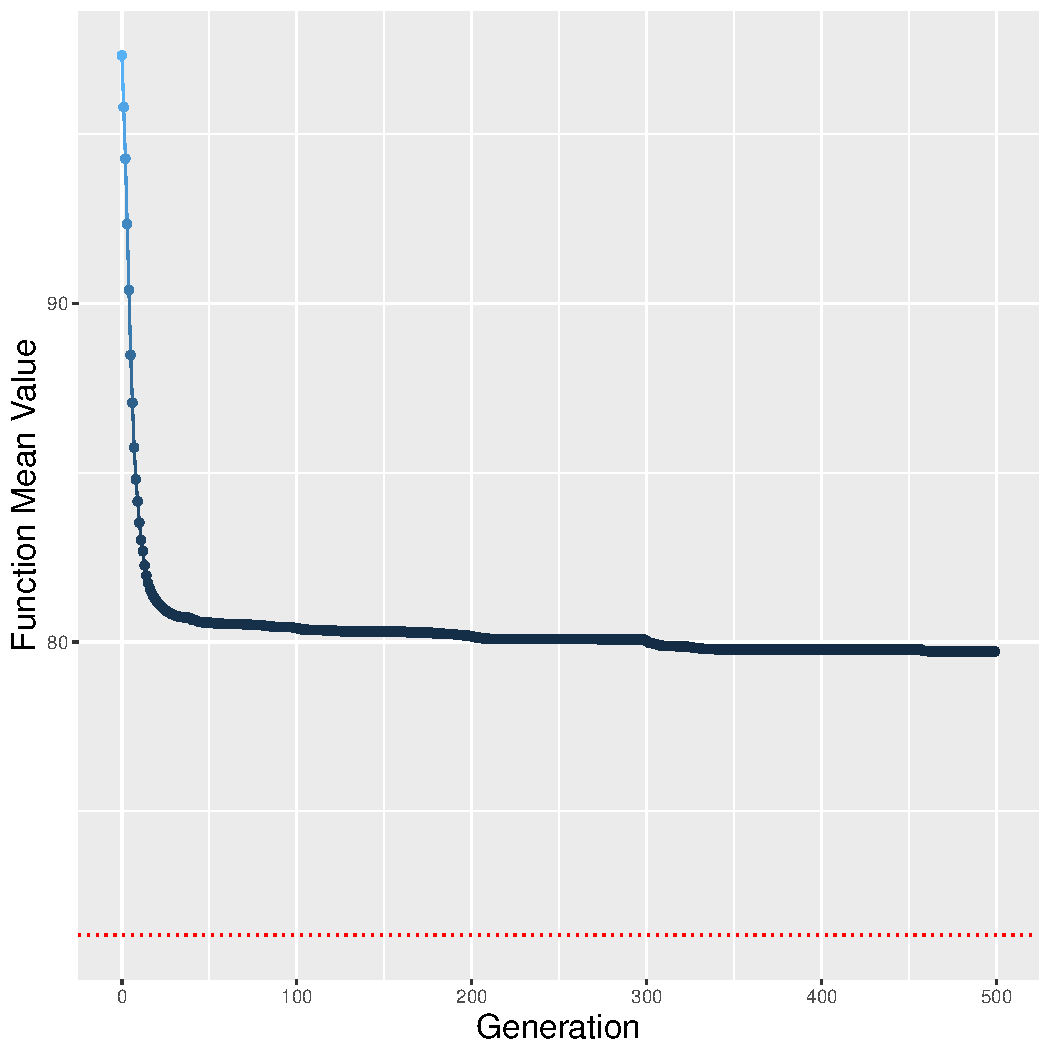
\includegraphics[width=\textwidth]{img/covergency_multimodal_2n2n_16_dim_20_tsize_16.pdf}
		\caption{Weierstrass Function with the SBX crossover - $(\lambda + \lambda)$ - 20 dimensions}
	\end{subfigure}
	\begin{subfigure}[b]{0.24\textwidth}
		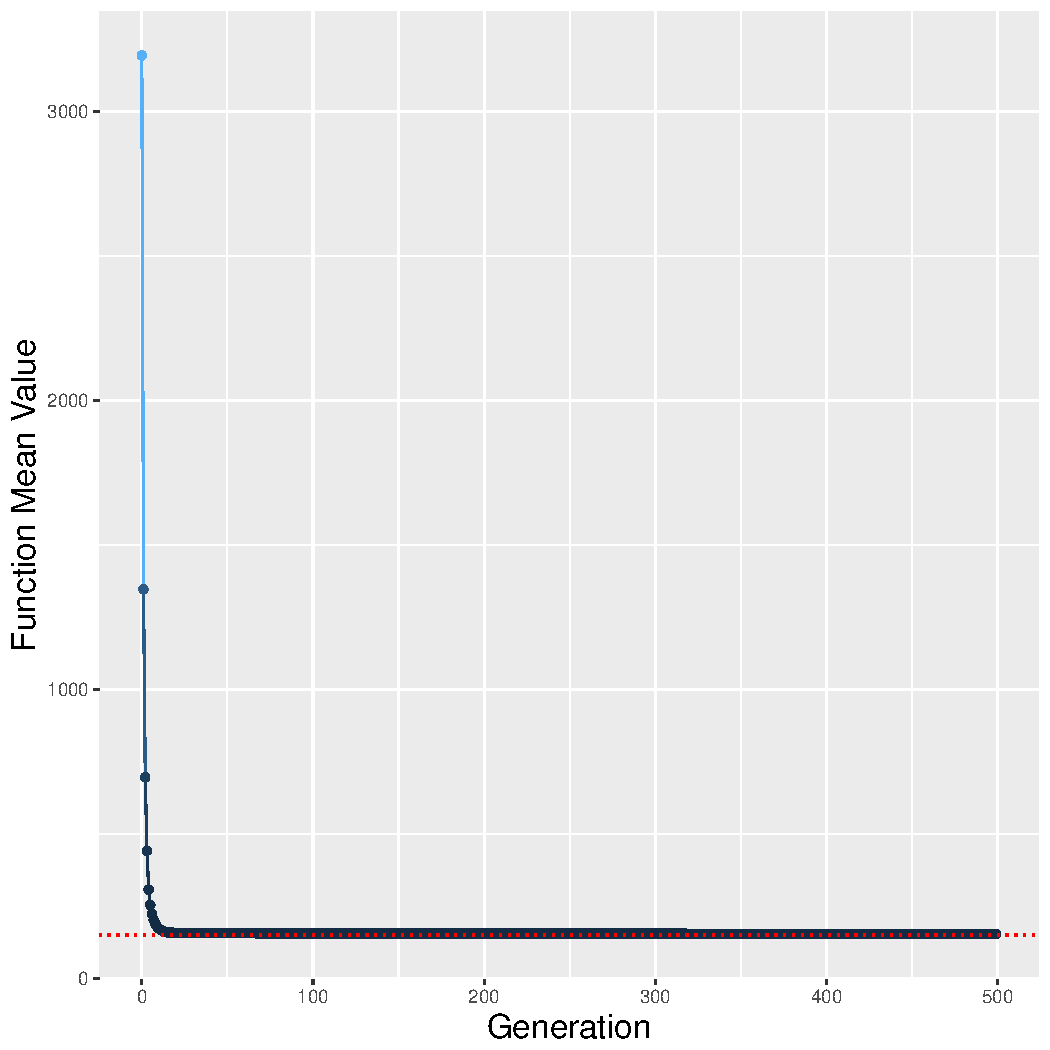
\includegraphics[width=\textwidth]{img/covergency_unimodal_sbx_8_dim_10_tsize_9.pdf}
		\caption{Rosenbrock Function - original with the SBX crossover - $(\lambda, \lambda)$ - 10 dimensions}
	\end{subfigure}
	\begin{subfigure}[b]{0.24\textwidth}
		\centering
		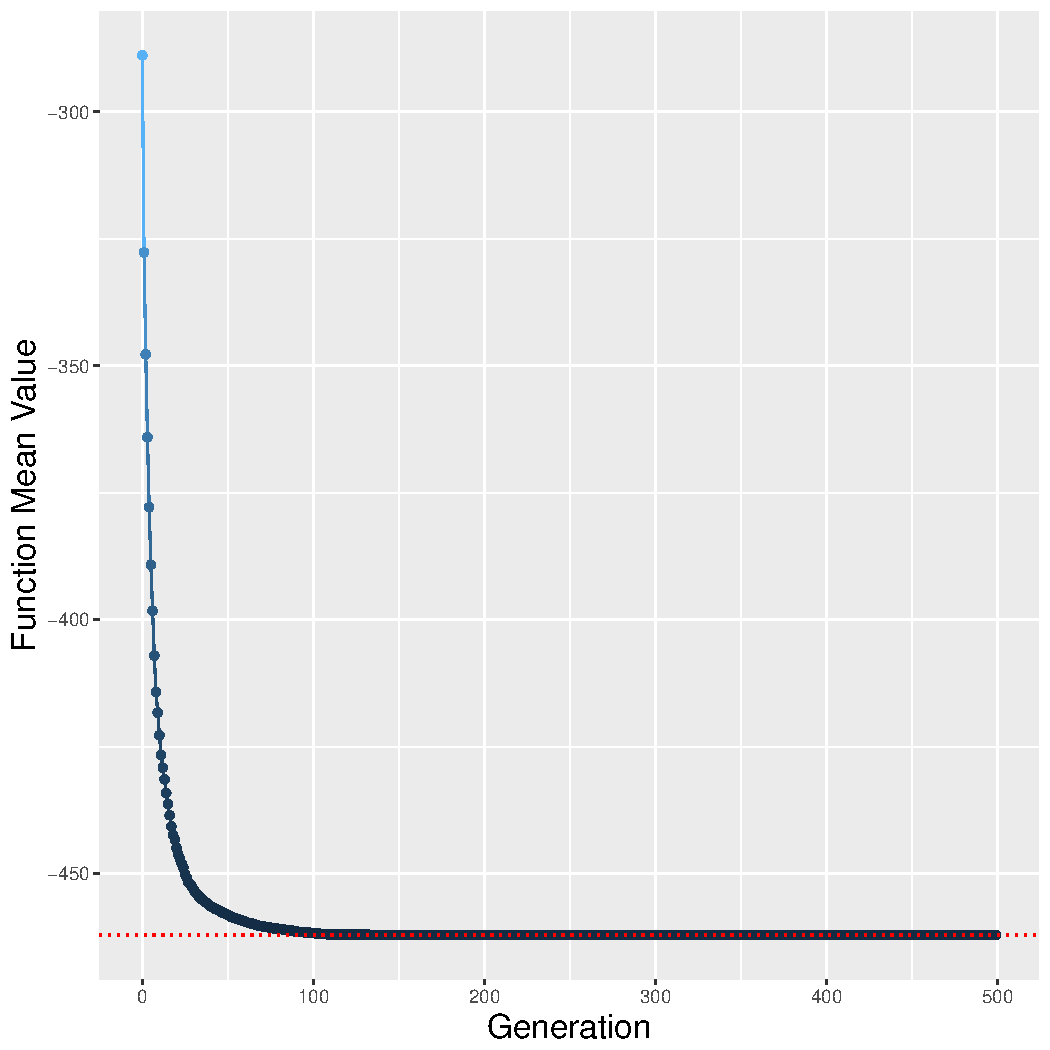
\includegraphics[width=\textwidth]{img/covergency_multimodal_sbx_4_dim_10_tsize_5.pdf}
		\caption{Buche-Rastrigin Function with the SBX crossover - $(\lambda + \lambda)$ - 10 dimensions}
	\end{subfigure}
	\begin{subfigure}[b]{0.24\textwidth}	
		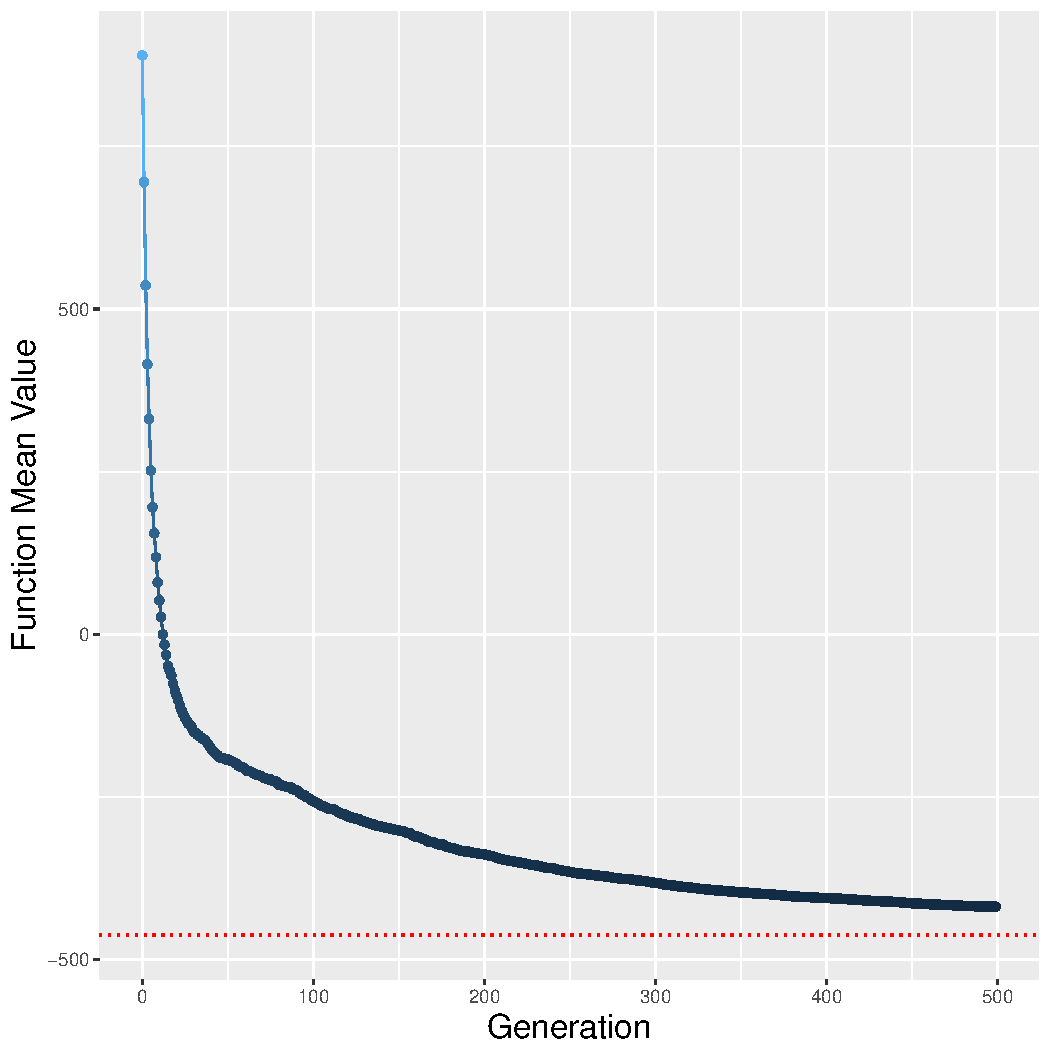
\includegraphics[width=\textwidth]{img/covergency_multimodal_sbx_3_dim_40_tsize_4.pdf}		
		\caption{Rastrigin Function with the SBX crossover - $(\lambda + \lambda)$ - 40 dimensions}
	\end{subfigure}
	\label{convergence}

	\caption{Examples of convergence for different \\combinations of functions and generational schemes.}
		\raggedright
\end{figure*}



\subsection{Overall Effect of K}

The Friedman Test showed no effect of changing the value of K
for unimodal functions with the uniform crossover and any
number of dimensions (Table~\ref{Friedman_test_uniform-a}). 

On the other hand, for unimodal functions with the SBX crossover, and
for multimodal functions with any other setup, the test indicated a
significant effect of changing the value of K on the final result of
the search~(Tables~\ref{Friedman_test_sbx-a}, \ref{Friedman_test_sbx-b}). 

An example of this effect can be seen in Figure~\ref{uniform-22-a},
where it is possible to see that for the Gallagher's Gaussian 21-hi
Peaks Function higher values for the tournament size indicate better
results.

\subsection{Analysis by Function}

To get a finer intuition of these results, we show some visual
examples separated in two groups of figures. The first group shows the
mean value achieved by the GA for the Gallagher's Gaussian 21-hi Peaks
Function, and the second group does the same for the Discus
Function. Both groups show the mean function values of 40 repetitions
for each set of parameters, and a linear regression line on the value
of K against the mean function value. While the results discussed here
are representative for the other functions studied, similar figures
for all other functions are available on the source repository.

Figures~\ref{sbx-22-a} and ~\ref{uniform-22-a} show that for the
Gallagher's Gaussian 21-hi Peaks Function (with 10, 20 and 40
dimensions) changing the tournament size to higher values tends to
increase the quality of the results for the generational scheme
($\lambda, \lambda$). On the other hand, for the generational scheme
($\lambda + \lambda$), Figure~\ref{sbx-22-B} shows that changing the
dimension has a dominating impact on the final values found by the
GA. This means that in this case the best tournament value depends on
the number of dimensions in the problem.

The dominance of the dimensionality observed in Figure~\ref{sbx-22-B}
also occurs in the Discus Function.
Figures~\ref{sbx-11-a},~\ref{uniform-11-a}, (with 10, 20 and 40
dimensions) show that changing the dimensionality of the problem may
have a high impact in the choice of the tournament value with the
generational scheme ($\lambda, \lambda$). Figure~\ref{sbx-11-B} shows
that with the generational scheme ($\lambda + \lambda$) changing the
tournament size leads to better final results. From these figures we
understand that smaller values positively affect the results,
specially with low dimensionality.

For all figures, the gray shaded area represents the 95\% confidence
level interval of a linear regression model. From these regressions,
we can see that sometimes choosing small values for K can be a poor
choice, a good choice, or make no difference at all. For all Figures,
the mean of 40 repetitions is shown as bullets and the red line at the
bottom shows the target value for the function.


\subsection{Convergence Assumption}

Finally, we want to make sure that all GA compositions used are actually
performing the search (even though the final effectiveness varies with
parameter choice). To verify this assumption, we perform a
visual examination of the convergence of the functions studied. 

Figure~\ref{convergence} is a selection of randomly samples of this
examination, namely the Weierstrass Function, the Rosenbrock Function
- original, the Buche-Rastrigin Function, and the Rastrigin Function
(F3), respectively.

From these figures we can see that the studied GAs are indeed
converging towards the optimum target value, represented by the bottom
red line. Similar figures for other GA/function combinations are
available on the source repository.

